% Options for packages loaded elsewhere
\PassOptionsToPackage{unicode}{hyperref}
\PassOptionsToPackage{hyphens}{url}
%
\documentclass[
]{book}
\usepackage{lmodern}
\usepackage{amssymb,amsmath}
\usepackage{ifxetex,ifluatex}
\ifnum 0\ifxetex 1\fi\ifluatex 1\fi=0 % if pdftex
  \usepackage[T1]{fontenc}
  \usepackage[utf8]{inputenc}
  \usepackage{textcomp} % provide euro and other symbols
\else % if luatex or xetex
  \usepackage{unicode-math}
  \defaultfontfeatures{Scale=MatchLowercase}
  \defaultfontfeatures[\rmfamily]{Ligatures=TeX,Scale=1}
\fi
% Use upquote if available, for straight quotes in verbatim environments
\IfFileExists{upquote.sty}{\usepackage{upquote}}{}
\IfFileExists{microtype.sty}{% use microtype if available
  \usepackage[]{microtype}
  \UseMicrotypeSet[protrusion]{basicmath} % disable protrusion for tt fonts
}{}
\makeatletter
\@ifundefined{KOMAClassName}{% if non-KOMA class
  \IfFileExists{parskip.sty}{%
    \usepackage{parskip}
  }{% else
    \setlength{\parindent}{0pt}
    \setlength{\parskip}{6pt plus 2pt minus 1pt}}
}{% if KOMA class
  \KOMAoptions{parskip=half}}
\makeatother
\usepackage{xcolor}
\IfFileExists{xurl.sty}{\usepackage{xurl}}{} % add URL line breaks if available
\IfFileExists{bookmark.sty}{\usepackage{bookmark}}{\usepackage{hyperref}}
\hypersetup{
  pdftitle={Polish Language(s) and Digital Humanities Using R},
  pdfauthor={G. Moroz},
  hidelinks,
  pdfcreator={LaTeX via pandoc}}
\urlstyle{same} % disable monospaced font for URLs
\usepackage{color}
\usepackage{fancyvrb}
\newcommand{\VerbBar}{|}
\newcommand{\VERB}{\Verb[commandchars=\\\{\}]}
\DefineVerbatimEnvironment{Highlighting}{Verbatim}{commandchars=\\\{\}}
% Add ',fontsize=\small' for more characters per line
\usepackage{framed}
\definecolor{shadecolor}{RGB}{248,248,248}
\newenvironment{Shaded}{\begin{snugshade}}{\end{snugshade}}
\newcommand{\AlertTok}[1]{\textcolor[rgb]{0.94,0.16,0.16}{#1}}
\newcommand{\AnnotationTok}[1]{\textcolor[rgb]{0.56,0.35,0.01}{\textbf{\textit{#1}}}}
\newcommand{\AttributeTok}[1]{\textcolor[rgb]{0.77,0.63,0.00}{#1}}
\newcommand{\BaseNTok}[1]{\textcolor[rgb]{0.00,0.00,0.81}{#1}}
\newcommand{\BuiltInTok}[1]{#1}
\newcommand{\CharTok}[1]{\textcolor[rgb]{0.31,0.60,0.02}{#1}}
\newcommand{\CommentTok}[1]{\textcolor[rgb]{0.56,0.35,0.01}{\textit{#1}}}
\newcommand{\CommentVarTok}[1]{\textcolor[rgb]{0.56,0.35,0.01}{\textbf{\textit{#1}}}}
\newcommand{\ConstantTok}[1]{\textcolor[rgb]{0.00,0.00,0.00}{#1}}
\newcommand{\ControlFlowTok}[1]{\textcolor[rgb]{0.13,0.29,0.53}{\textbf{#1}}}
\newcommand{\DataTypeTok}[1]{\textcolor[rgb]{0.13,0.29,0.53}{#1}}
\newcommand{\DecValTok}[1]{\textcolor[rgb]{0.00,0.00,0.81}{#1}}
\newcommand{\DocumentationTok}[1]{\textcolor[rgb]{0.56,0.35,0.01}{\textbf{\textit{#1}}}}
\newcommand{\ErrorTok}[1]{\textcolor[rgb]{0.64,0.00,0.00}{\textbf{#1}}}
\newcommand{\ExtensionTok}[1]{#1}
\newcommand{\FloatTok}[1]{\textcolor[rgb]{0.00,0.00,0.81}{#1}}
\newcommand{\FunctionTok}[1]{\textcolor[rgb]{0.00,0.00,0.00}{#1}}
\newcommand{\ImportTok}[1]{#1}
\newcommand{\InformationTok}[1]{\textcolor[rgb]{0.56,0.35,0.01}{\textbf{\textit{#1}}}}
\newcommand{\KeywordTok}[1]{\textcolor[rgb]{0.13,0.29,0.53}{\textbf{#1}}}
\newcommand{\NormalTok}[1]{#1}
\newcommand{\OperatorTok}[1]{\textcolor[rgb]{0.81,0.36,0.00}{\textbf{#1}}}
\newcommand{\OtherTok}[1]{\textcolor[rgb]{0.56,0.35,0.01}{#1}}
\newcommand{\PreprocessorTok}[1]{\textcolor[rgb]{0.56,0.35,0.01}{\textit{#1}}}
\newcommand{\RegionMarkerTok}[1]{#1}
\newcommand{\SpecialCharTok}[1]{\textcolor[rgb]{0.00,0.00,0.00}{#1}}
\newcommand{\SpecialStringTok}[1]{\textcolor[rgb]{0.31,0.60,0.02}{#1}}
\newcommand{\StringTok}[1]{\textcolor[rgb]{0.31,0.60,0.02}{#1}}
\newcommand{\VariableTok}[1]{\textcolor[rgb]{0.00,0.00,0.00}{#1}}
\newcommand{\VerbatimStringTok}[1]{\textcolor[rgb]{0.31,0.60,0.02}{#1}}
\newcommand{\WarningTok}[1]{\textcolor[rgb]{0.56,0.35,0.01}{\textbf{\textit{#1}}}}
\usepackage{longtable,booktabs}
% Correct order of tables after \paragraph or \subparagraph
\usepackage{etoolbox}
\makeatletter
\patchcmd\longtable{\par}{\if@noskipsec\mbox{}\fi\par}{}{}
\makeatother
% Allow footnotes in longtable head/foot
\IfFileExists{footnotehyper.sty}{\usepackage{footnotehyper}}{\usepackage{footnote}}
\makesavenoteenv{longtable}
\usepackage{graphicx,grffile}
\makeatletter
\def\maxwidth{\ifdim\Gin@nat@width>\linewidth\linewidth\else\Gin@nat@width\fi}
\def\maxheight{\ifdim\Gin@nat@height>\textheight\textheight\else\Gin@nat@height\fi}
\makeatother
% Scale images if necessary, so that they will not overflow the page
% margins by default, and it is still possible to overwrite the defaults
% using explicit options in \includegraphics[width, height, ...]{}
\setkeys{Gin}{width=\maxwidth,height=\maxheight,keepaspectratio}
% Set default figure placement to htbp
\makeatletter
\def\fps@figure{htbp}
\makeatother
\setlength{\emergencystretch}{3em} % prevent overfull lines
\providecommand{\tightlist}{%
  \setlength{\itemsep}{0pt}\setlength{\parskip}{0pt}}
\setcounter{secnumdepth}{5}
\usepackage{booktabs}
\makeatletter
\newenvironment{kframe}{%
\medskip{}
\setlength{\fboxsep}{.8em}
 \def\at@end@of@kframe{}%
 \ifinner\ifhmode%
  \def\at@end@of@kframe{\end{minipage}}%
  \begin{minipage}{\columnwidth}%
 \fi\fi%
 \def\FrameCommand##1{\hskip\@totalleftmargin \hskip-\fboxsep
 \colorbox{shadecolor}{##1}\hskip-\fboxsep
     % There is no \\@totalrightmargin, so:
     \hskip-\linewidth \hskip-\@totalleftmargin \hskip\columnwidth}%
 \MakeFramed {\advance\hsize-\width
   \@totalleftmargin\z@ \linewidth\hsize
   \@setminipage}}%
 {\par\unskip\endMakeFramed%
 \at@end@of@kframe}
\makeatother

\makeatletter
\@ifundefined{Shaded}{
}{\renewenvironment{Shaded}{\begin{kframe}}{\end{kframe}}}
\makeatother
\newenvironment{rmdblock}[1]
  {
  \begin{itemize}
  \renewcommand{\labelitemi}{
    \raisebox{-.7\height}[0pt][0pt]{
      {\setkeys{Gin}{width=3em,keepaspectratio}\includegraphics{images/#1}}
    }
  }
  \setlength{\fboxsep}{1em}
  \begin{kframe}
  \item
  }
  {
  \end{kframe}
  \end{itemize}
  }
\newenvironment{rmdtask}
  {\begin{rmdblock}{task}}
  {\end{rmdblock}}
\usepackage[]{natbib}
\bibliographystyle{apalike}

\title{Polish Language(s) and Digital Humanities Using R}
\author{G. Moroz}
\date{2020}

\begin{document}
\frontmatter
\maketitle

{
\setcounter{tocdepth}{1}
\tableofcontents
}
\mainmatter
\hypertarget{prerequisites}{%
\chapter{Prerequisites}\label{prerequisites}}

Before the classes I would like to ask you to follow the instructions mentioned below to prepare your device for the class work:

\begin{itemize}
\tightlist
\item
  install \textbf{R} from the following link: \url{https://cloud.r-project.org/}
\item
  install \textbf{RStudio} from the following link: \url{https://rstudio.com/products/rstudio/download/\#download} (FREE version, no need to pay!)
\item
  after the installation run the RStudio program, type \texttt{2+2}, and press \texttt{Enter}.
\end{itemize}

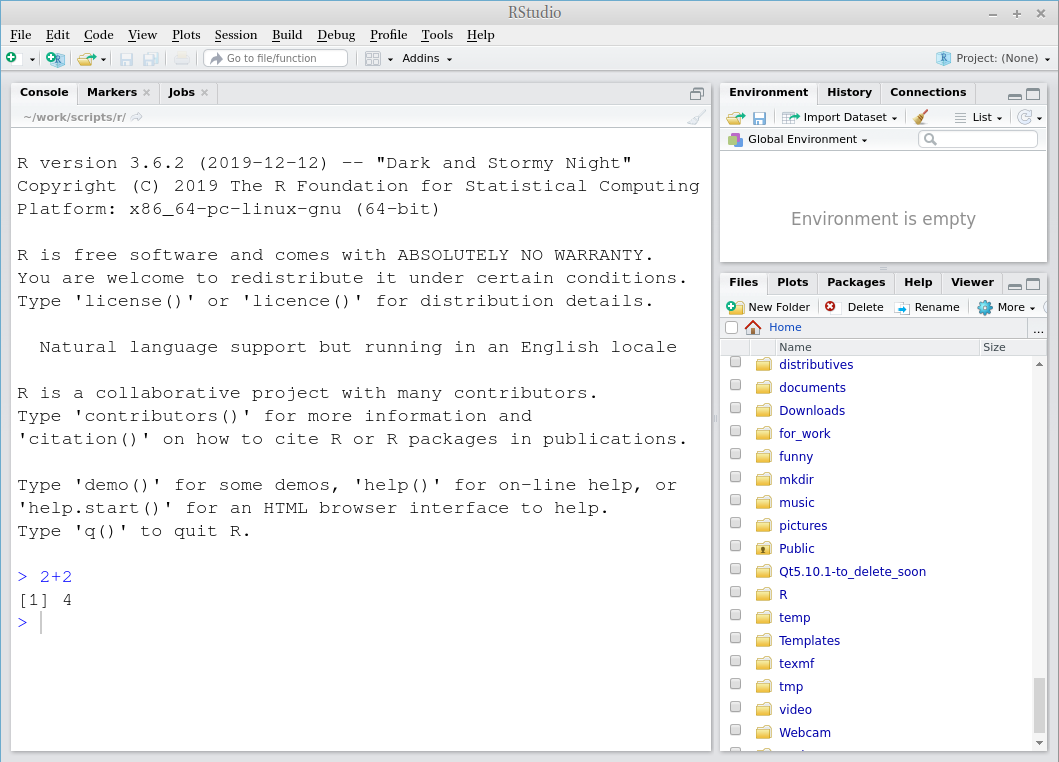
\includegraphics{images/00.rstudio-view.png}

If you see something like this, then you are well prepared for classes.

\begin{itemize}
\tightlist
\item
  Go to the \url{https://rstudio.cloud/} website and sign up there. This is optional, but it will be a backup version, if something will not work on your computer.
\end{itemize}

\hypertarget{intro}{%
\chapter{Introduction to R and RStudio}\label{intro}}

\hypertarget{introduction}{%
\section{Introduction}\label{introduction}}

\hypertarget{why-data-science}{%
\subsection{Why data science?}\label{why-data-science}}

Data science is a new field that actively developing lately. This field merges computer science, math, statistics, and it is hard to say how much science in data science. In many scientific fields a new data science paradigm arises and even forms a new sub-field:

\begin{itemize}
\tightlist
\item
  Bioinformatics
\item
  Crime data analysis
\item
  Digital humanities
\item
  Data journalism
\item
  Data driven medicine
\item
  \ldots{}
\end{itemize}

There are a lot of new books ``Data Science for \ldots{}'':

\begin{itemize}
\tightlist
\item
  psychologists \citep{hansjoerg19}
\item
  immunologists \citep{thomas19}
\item
  business \citep{provost13}
\item
  public policy \citep{brooks13}
\item
  fraud detection \citep{baesens15}
\item
  \ldots{}
\end{itemize}

Data scientist need to be able:

\begin{itemize}
\tightlist
\item
  gather data
\item
  transform data
\item
  visualize data
\item
  create a statistical model based on data
\item
  share and represent the results of this work
\item
  organize the whole workflow in the reproducible way
\end{itemize}

\hypertarget{why-r}{%
\subsection{Why R?}\label{why-r}}

R \citep{r19} is a programming language with a big infrastructure of packages that helps to work in different fields of science and computer technology.

There are several alternatives:

\begin{itemize}
\tightlist
\item
  Python \citep{vanderplas16, grus19}
\item
  Julia \citep{bezanson17}
\item
  bash \citep{janssens14}
\item
  java \citep{brzustowicz17}
\item
  \ldots{}
\end{itemize}

You can find some R answers here:

\begin{itemize}
\tightlist
\item
  R for data science \citep{wickham16}, it is online
\item
  \href{https://community.rstudio.com/}{R community}
\item
  \href{https://stackoverflow.com}{stackoverflow}
\item
  any search engine you use
\item
  \ldots{}
\end{itemize}

\hypertarget{introduction-to-rstudio}{%
\section{Introduction to RStudio}\label{introduction-to-rstudio}}

R is the programming language. RStudio is the most popular IDE (Integrated Development Environment) for R language.

When you open RStudio for the first time you can see something like this:

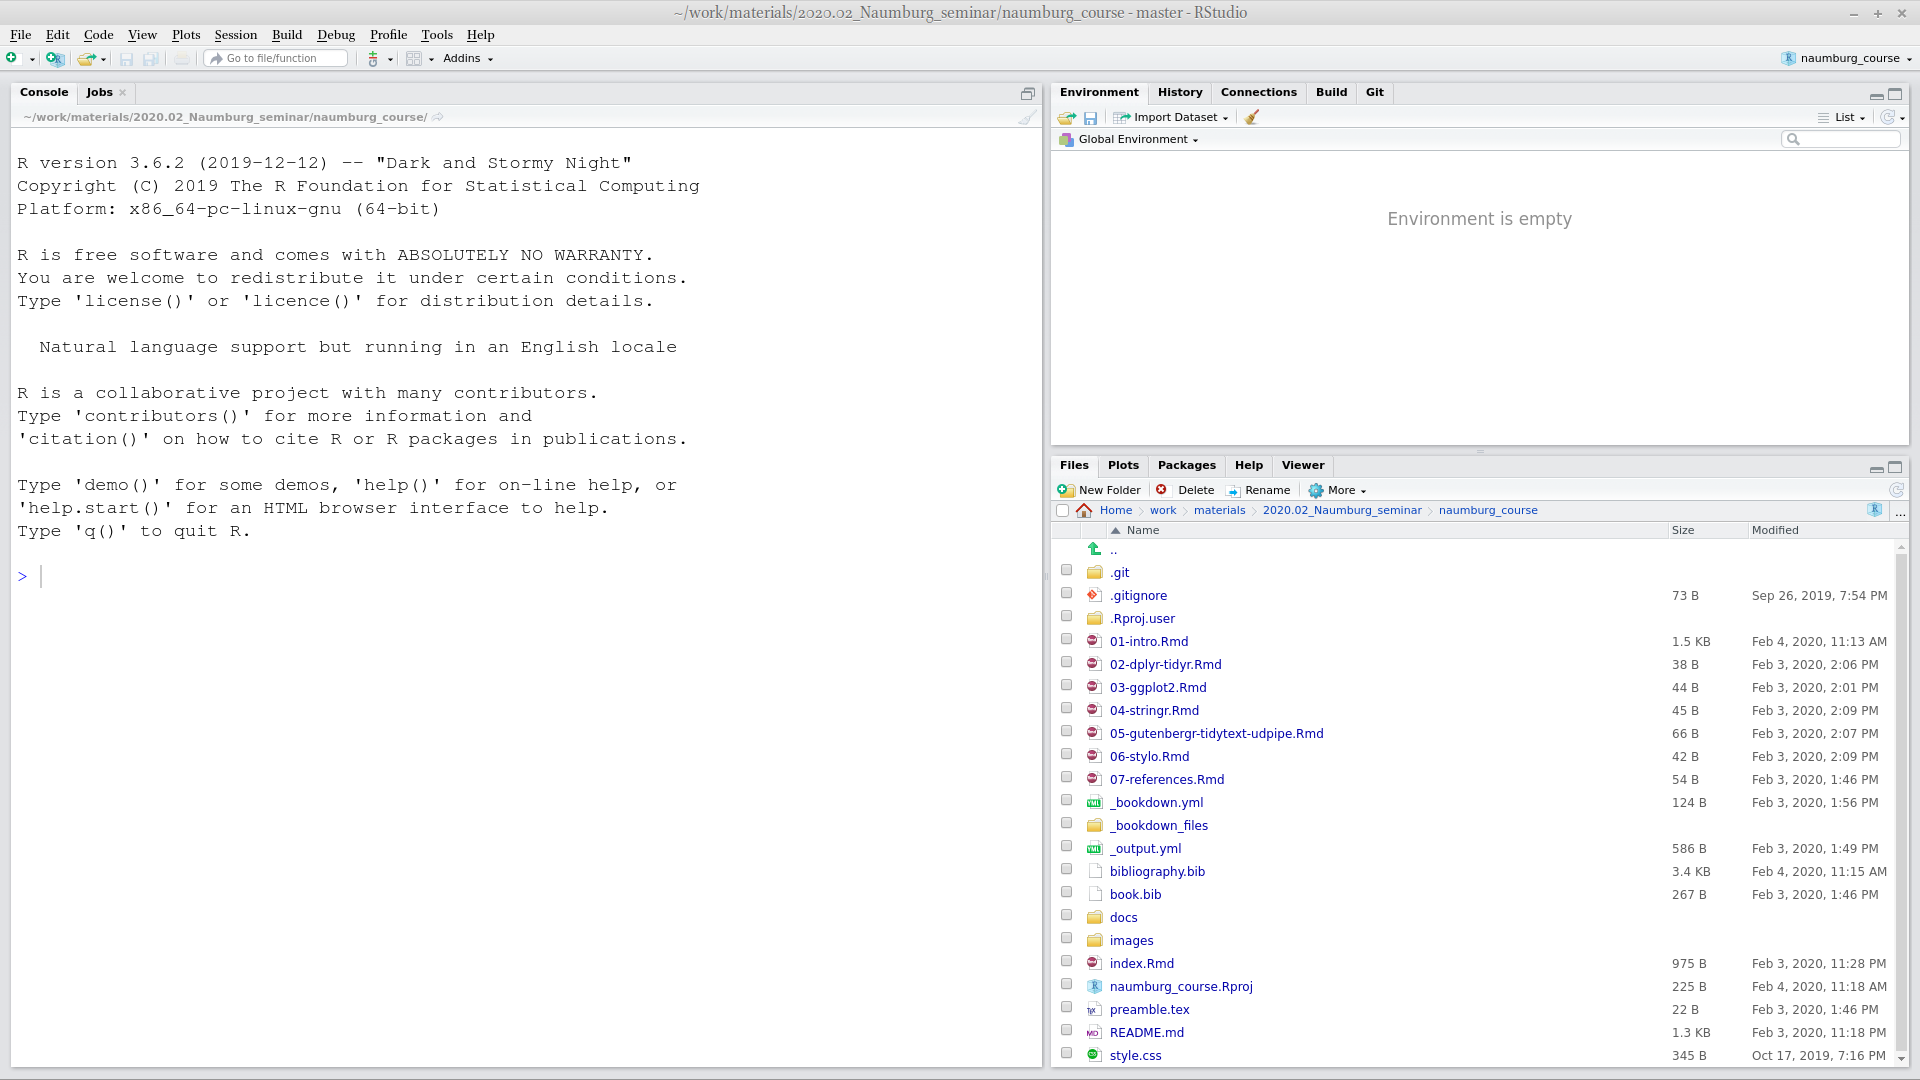
\includegraphics{images/01.01.rstudio.png}

When you press 
\includegraphics{images/01.02.rstudio_button.png} button at the top of the left window you will be able to see all four panels of the RStudio.

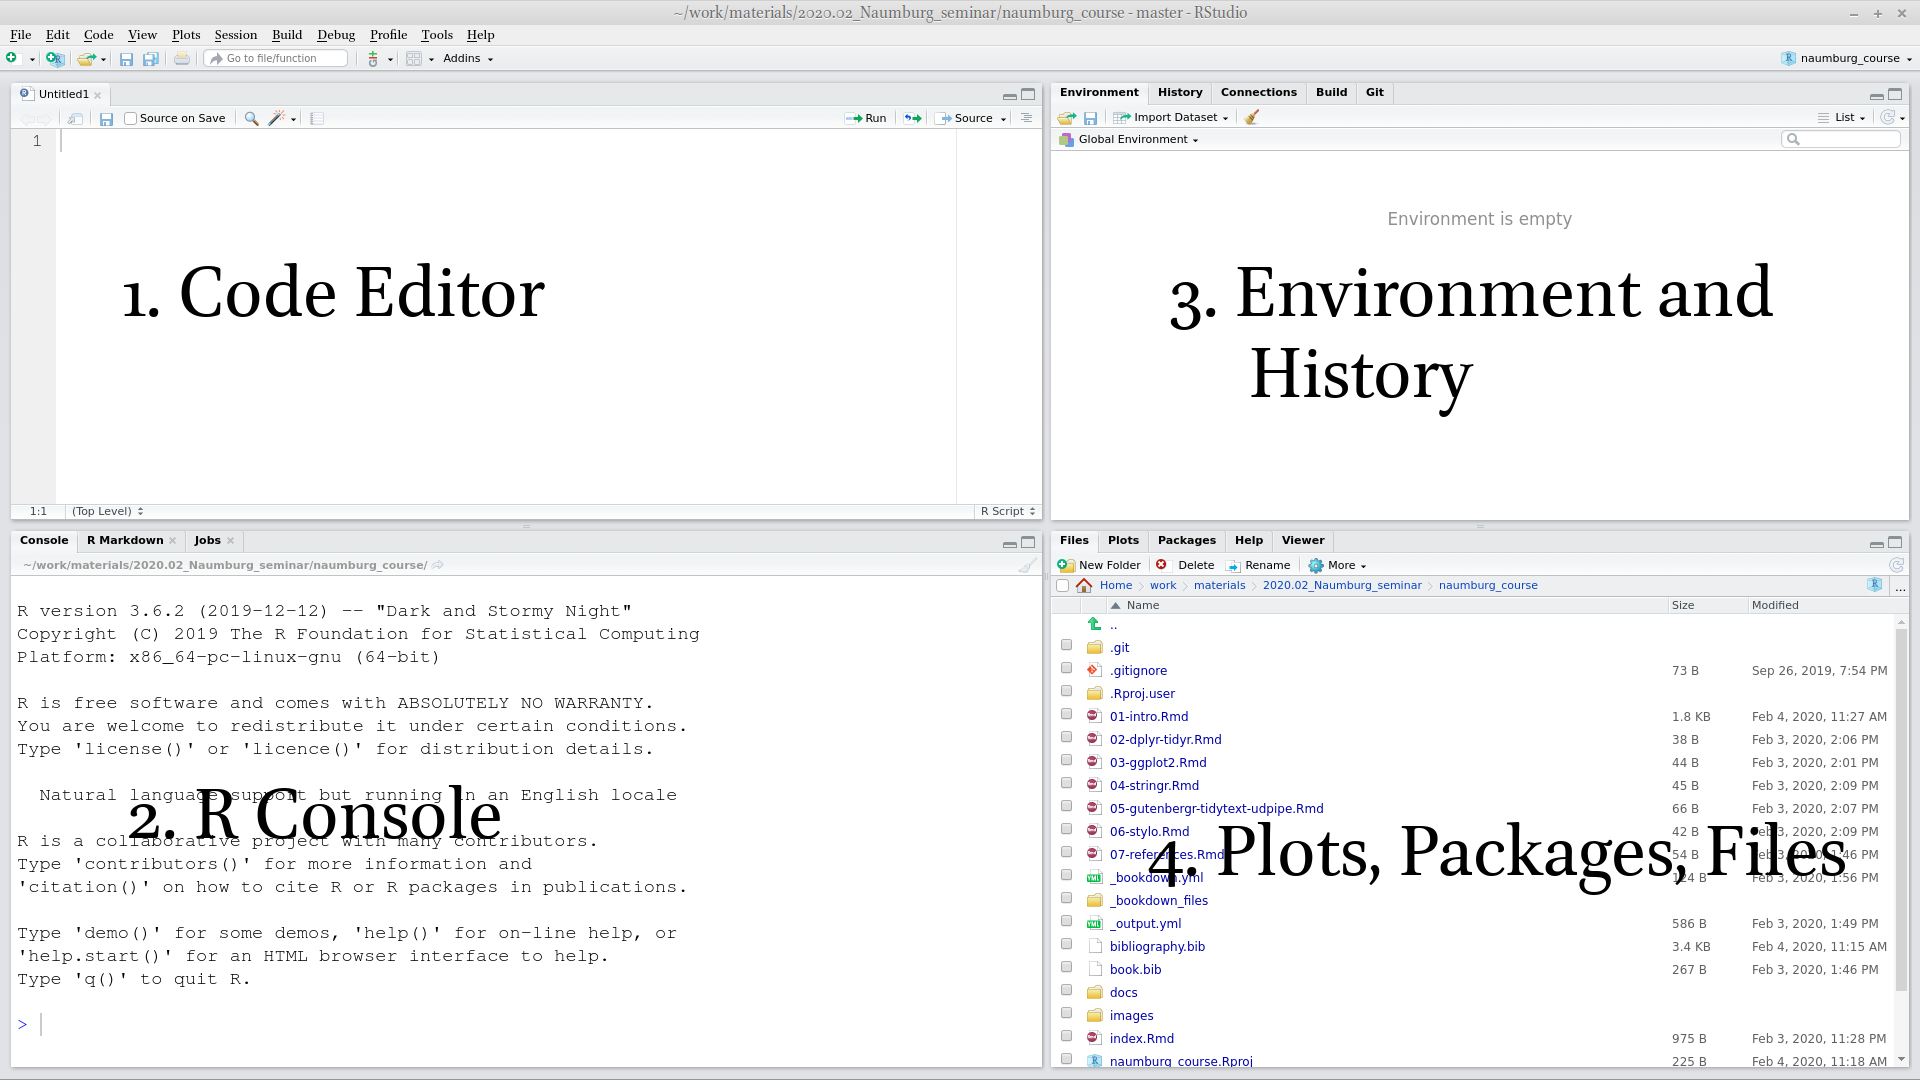
\includegraphics{images/01.03.rstudio.png}

\hypertarget{r-as-a-calculator}{%
\section{R as a calculator}\label{r-as-a-calculator}}

Lets first start with a calculator. Press in R console

\begin{Shaded}
\begin{Highlighting}[]
\DecValTok{2}\OperatorTok{+}\DecValTok{9}
\end{Highlighting}
\end{Shaded}

\begin{verbatim}
## [1] 11
\end{verbatim}

\begin{Shaded}
\begin{Highlighting}[]
\DecValTok{50}\OperatorTok{*}\NormalTok{(}\DecValTok{9-20}\NormalTok{)}
\end{Highlighting}
\end{Shaded}

\begin{verbatim}
## [1] -550
\end{verbatim}

\begin{Shaded}
\begin{Highlighting}[]
\DecValTok{3}\OperatorTok{^}\DecValTok{3}
\end{Highlighting}
\end{Shaded}

\begin{verbatim}
## [1] 27
\end{verbatim}

\begin{Shaded}
\begin{Highlighting}[]
\DecValTok{9}\OperatorTok{^}\FloatTok{0.5}
\end{Highlighting}
\end{Shaded}

\begin{verbatim}
## [1] 3
\end{verbatim}

\begin{Shaded}
\begin{Highlighting}[]
\DecValTok{9}\FloatTok{+0.5}
\end{Highlighting}
\end{Shaded}

\begin{verbatim}
## [1] 9.5
\end{verbatim}

\begin{Shaded}
\begin{Highlighting}[]
\DecValTok{9}\FloatTok{+.5}
\end{Highlighting}
\end{Shaded}

\begin{verbatim}
## [1] 9.5
\end{verbatim}

\begin{Shaded}
\begin{Highlighting}[]
\NormalTok{pi}
\end{Highlighting}
\end{Shaded}

\begin{verbatim}
## [1] 3.141593
\end{verbatim}

Reminder after division

\begin{Shaded}
\begin{Highlighting}[]
\DecValTok{10} \OperatorTok\StringTok{ }\DecValTok{3}
\end{Highlighting}
\end{Shaded}

\begin{verbatim}
## [1] 1
\end{verbatim}

\begin{rmdtask}
So you are ready to solve some really hard equations (round it four
decimal places):
\end{rmdtask}

\[\frac{\pi+2}{2^{3-\pi}}\]

📋 list of hints ➡

👁 Are you sure that you rounded the result? ➡
I expect the answer to be rounded to four decimal places: \texttt{0.87654321} becomes \texttt{0.8765}.

👁 Are you sure you didn't get into the brackets trap? ➡
Even though there is no any brackets in the mathematical notation, you need to add them in R, otherwise the operation order will be wrong.

\hypertarget{comments}{%
\section{Comments}\label{comments}}

All text after the hash \texttt{\#} within the same line is considered a comment.

\begin{Shaded}
\begin{Highlighting}[]
\DecValTok{2}\OperatorTok{+}\DecValTok{2} \CommentTok{# it is four}
\end{Highlighting}
\end{Shaded}

\begin{verbatim}
## [1] 4
\end{verbatim}

\begin{Shaded}
\begin{Highlighting}[]
\CommentTok{# you can put any comments here}
\DecValTok{3}\OperatorTok{+}\DecValTok{3}
\end{Highlighting}
\end{Shaded}

\begin{verbatim}
## [1] 6
\end{verbatim}

\hypertarget{functions}{%
\section{Functions}\label{functions}}

The most important part of R is functions: here are some of them:

\begin{Shaded}
\begin{Highlighting}[]
\KeywordTok{sqrt}\NormalTok{(}\DecValTok{4}\NormalTok{)}
\end{Highlighting}
\end{Shaded}

\begin{verbatim}
## [1] 2
\end{verbatim}

\begin{Shaded}
\begin{Highlighting}[]
\KeywordTok{abs}\NormalTok{(}\OperatorTok{-}\DecValTok{5}\NormalTok{)}
\end{Highlighting}
\end{Shaded}

\begin{verbatim}
## [1] 5
\end{verbatim}

\begin{Shaded}
\begin{Highlighting}[]
\KeywordTok{sin}\NormalTok{(pi}\OperatorTok{/}\DecValTok{2}\NormalTok{)}
\end{Highlighting}
\end{Shaded}

\begin{verbatim}
## [1] 1
\end{verbatim}

\begin{Shaded}
\begin{Highlighting}[]
\KeywordTok{cos}\NormalTok{(pi)}
\end{Highlighting}
\end{Shaded}

\begin{verbatim}
## [1] -1
\end{verbatim}

\begin{Shaded}
\begin{Highlighting}[]
\KeywordTok{sum}\NormalTok{(}\DecValTok{2}\NormalTok{, }\DecValTok{3}\NormalTok{, }\DecValTok{9}\NormalTok{)}
\end{Highlighting}
\end{Shaded}

\begin{verbatim}
## [1] 14
\end{verbatim}

\begin{Shaded}
\begin{Highlighting}[]
\KeywordTok{prod}\NormalTok{(}\DecValTok{5}\NormalTok{, }\DecValTok{3}\NormalTok{, }\DecValTok{9}\NormalTok{)}
\end{Highlighting}
\end{Shaded}

\begin{verbatim}
## [1] 135
\end{verbatim}

\begin{Shaded}
\begin{Highlighting}[]
\KeywordTok{sin}\NormalTok{(}\KeywordTok{cos}\NormalTok{(pi))}
\end{Highlighting}
\end{Shaded}

\begin{verbatim}
## [1] -0.841471
\end{verbatim}

Each function has a name and zero or more arguments. All arguments of the function should be listed in parenthesis and separated by comma:

\begin{Shaded}
\begin{Highlighting}[]
\NormalTok{pi}
\end{Highlighting}
\end{Shaded}

\begin{verbatim}
## [1] 3.141593
\end{verbatim}

\begin{Shaded}
\begin{Highlighting}[]
\KeywordTok{round}\NormalTok{(pi, }\DecValTok{2}\NormalTok{)}
\end{Highlighting}
\end{Shaded}

\begin{verbatim}
## [1] 3.14
\end{verbatim}

Each function's argument has its own name and serial number. If you use names of the function's arguments, you can put them in any order. If you do not use names of the function's arguments, you should put them according the serial number.

\begin{Shaded}
\begin{Highlighting}[]
\KeywordTok{round}\NormalTok{(}\DataTypeTok{x =}\NormalTok{ pi, }\DataTypeTok{digits =} \DecValTok{2}\NormalTok{)}
\end{Highlighting}
\end{Shaded}

\begin{verbatim}
## [1] 3.14
\end{verbatim}

\begin{Shaded}
\begin{Highlighting}[]
\KeywordTok{round}\NormalTok{(}\DataTypeTok{digits =} \DecValTok{2}\NormalTok{, }\DataTypeTok{x =}\NormalTok{ pi)}
\end{Highlighting}
\end{Shaded}

\begin{verbatim}
## [1] 3.14
\end{verbatim}

\begin{Shaded}
\begin{Highlighting}[]
\KeywordTok{round}\NormalTok{(}\DataTypeTok{x =}\NormalTok{ pi, }\DataTypeTok{d =} \DecValTok{2}\NormalTok{)}
\end{Highlighting}
\end{Shaded}

\begin{verbatim}
## [1] 3.14
\end{verbatim}

\begin{Shaded}
\begin{Highlighting}[]
\KeywordTok{round}\NormalTok{(}\DataTypeTok{d =} \DecValTok{2}\NormalTok{, }\DataTypeTok{x =}\NormalTok{ pi)}
\end{Highlighting}
\end{Shaded}

\begin{verbatim}
## [1] 3.14
\end{verbatim}

\begin{Shaded}
\begin{Highlighting}[]
\KeywordTok{round}\NormalTok{(pi, }\DecValTok{2}\NormalTok{)}
\end{Highlighting}
\end{Shaded}

\begin{verbatim}
## [1] 3.14
\end{verbatim}

\begin{Shaded}
\begin{Highlighting}[]
\KeywordTok{round}\NormalTok{(}\DecValTok{2}\NormalTok{, pi) }\CommentTok{# this is not the same as all previouse!}
\end{Highlighting}
\end{Shaded}

\begin{verbatim}
## [1] 2
\end{verbatim}

There are some functions without any arguments, but you still should use parenthesis:

\begin{Shaded}
\begin{Highlighting}[]
\KeywordTok{Sys.Date}\NormalTok{() }\CommentTok{# correct}
\end{Highlighting}
\end{Shaded}

\begin{verbatim}
## [1] "2020-02-05"
\end{verbatim}

\begin{Shaded}
\begin{Highlighting}[]
\NormalTok{Sys.Date }\CommentTok{# wrong}
\end{Highlighting}
\end{Shaded}

\begin{verbatim}
## function () 
## as.Date(as.POSIXlt(Sys.time()))
## <bytecode: 0x625bf08cc528>
## <environment: namespace:base>
\end{verbatim}

Each function in R is documented. You can read its documentation typing question mark before the function name:

\begin{Shaded}
\begin{Highlighting}[]
\NormalTok{?Sys.Date}
\end{Highlighting}
\end{Shaded}

\begin{rmdtask}
Explore the function \texttt{log()} and calculate the following
logarithm:
\end{rmdtask}

\[\log_3(3486784401)\]

📋 list of hints ➡

👁 A-a-a! I don't remember anything about logarithms\ldots{} ➡
The logarithm is the inverse function to exponentiation. That means the logarithm of a given number \emph{x} is the exponent to which another fixed number, the base \emph{b}, must be raised, to produce that number \emph{x}.

\[10^n = 1000,\text{ what is n?}\]
\[n = \log_{10}(1000)\]

👁 What is this small 3 in the task means? ➡
This is the base of the logarithm. So the task is: what is the exponent to which another fixed number, the base \emph{3}, must be raised, to produce that number \emph{3486784401}.

\hypertarget{variables}{%
\section{Variables}\label{variables}}

Everything in R can be stored in a variable:

\begin{Shaded}
\begin{Highlighting}[]
\NormalTok{x <-}\StringTok{ }\DecValTok{5} \OperatorTok{+}\StringTok{ }\DecValTok{6}
\end{Highlighting}
\end{Shaded}

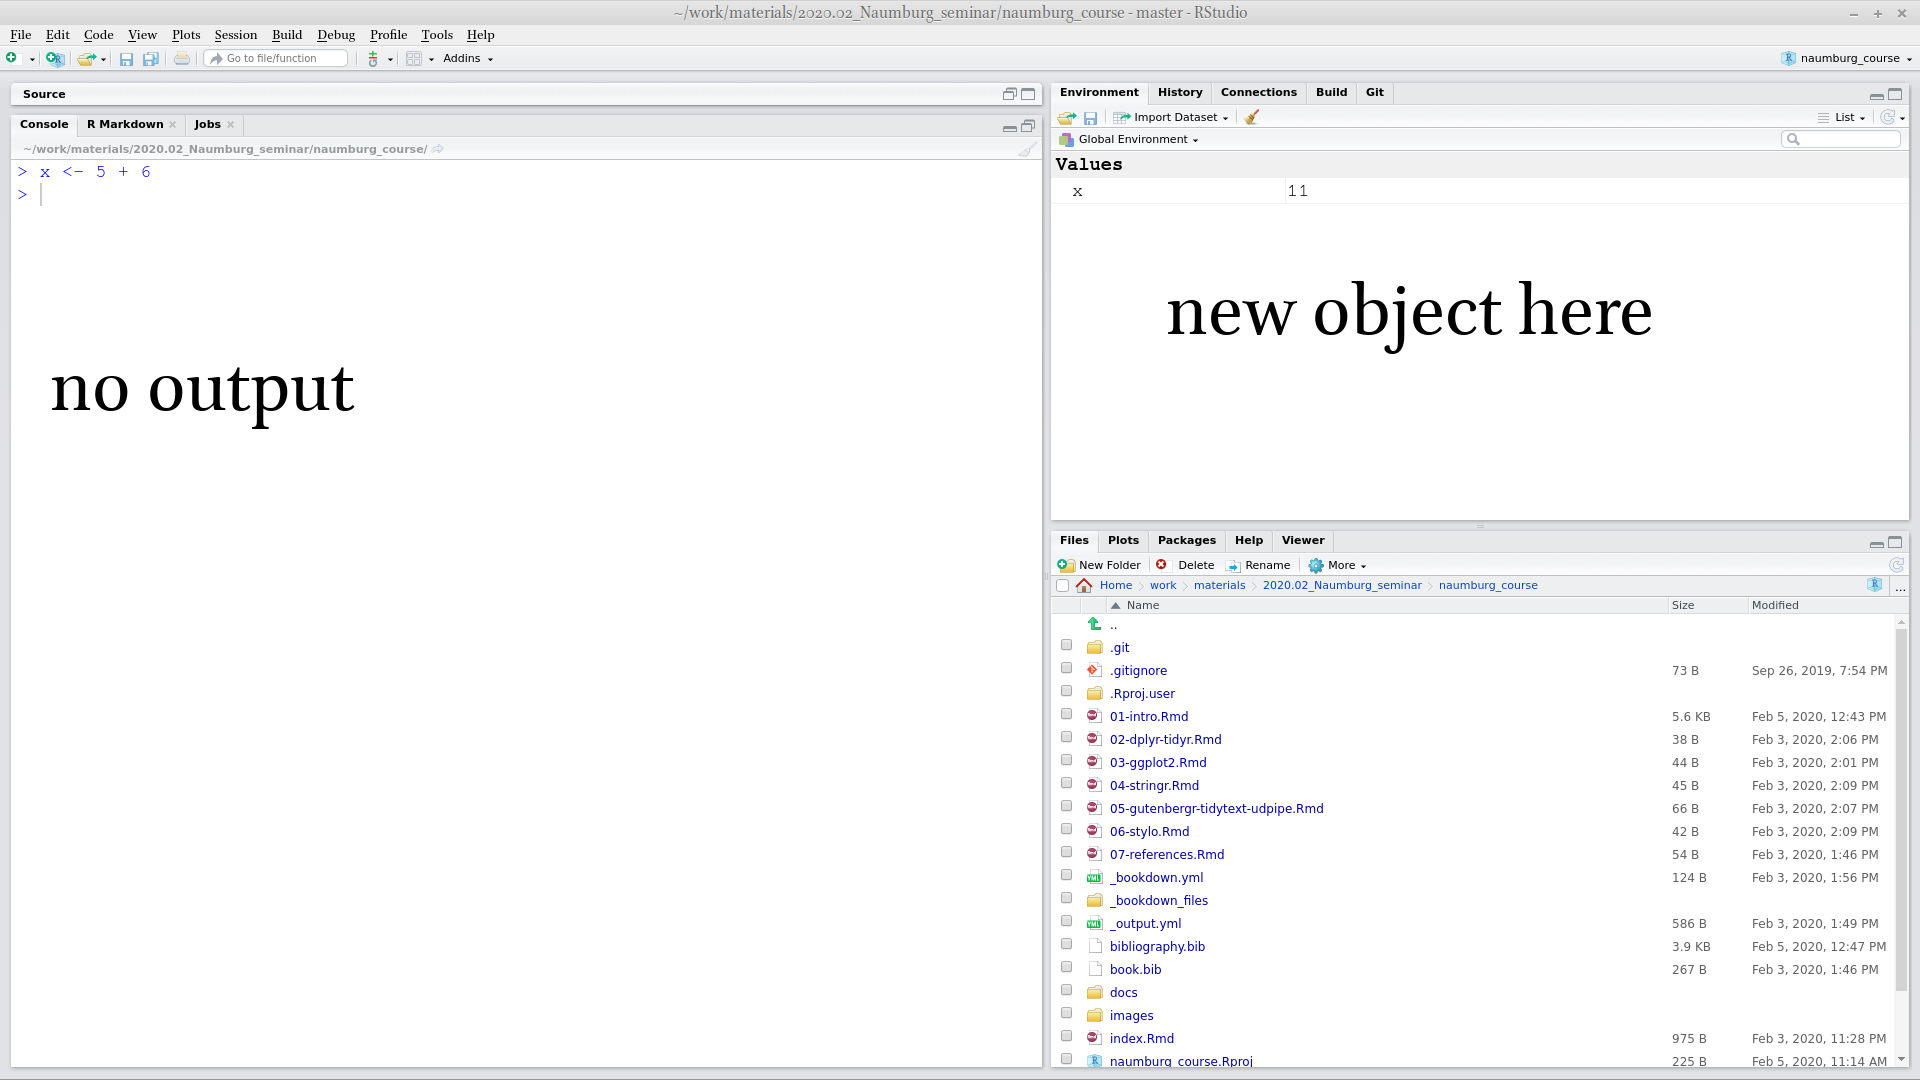
\includegraphics{images/01.04.variable.png}
As a result, no output in the Console, and a new variable \emph{x} appear in the Environment window. From now on I can use this new variable:

\begin{Shaded}
\begin{Highlighting}[]
\NormalTok{x }\OperatorTok{+}\StringTok{ }\NormalTok{x}
\end{Highlighting}
\end{Shaded}

\begin{verbatim}
## [1] 22
\end{verbatim}

\begin{Shaded}
\begin{Highlighting}[]
\KeywordTok{sum}\NormalTok{(x, x, }\DecValTok{7}\NormalTok{)}
\end{Highlighting}
\end{Shaded}

\begin{verbatim}
## [1] 29
\end{verbatim}

All those operation don't change the variable value. In order to change the variable value you need to make a new assignment:

\begin{Shaded}
\begin{Highlighting}[]
\NormalTok{x <-}\StringTok{ }\DecValTok{5} \OperatorTok{+}\StringTok{ }\DecValTok{6} \OperatorTok{+}\StringTok{ }\DecValTok{7}
\end{Highlighting}
\end{Shaded}

The fast way for creating \texttt{\textless{}-} in RStudio is to press \texttt{Alt\ -} on your keyboard.

It is possible to use equal sign \texttt{=} for assignment operation, but the recommendations are use arrow \texttt{\textless{}-} for the assignment, and equal sign \texttt{=} for giving arguments' value inside the functions.

For removing vector you need to use function \texttt{rm()}:

\begin{Shaded}
\begin{Highlighting}[]
\KeywordTok{rm}\NormalTok{(x)}
\NormalTok{x}
\end{Highlighting}
\end{Shaded}

\begin{verbatim}
## Error in eval(expr, envir, enclos): object 'x' not found
\end{verbatim}

\hypertarget{variable-comparison}{%
\subsection{Variable comparison}\label{variable-comparison}}

It is possible to compare different variables

\begin{Shaded}
\begin{Highlighting}[]
\NormalTok{x <-}\StringTok{ }\DecValTok{18}
\NormalTok{x }\OperatorTok{>}\StringTok{ }\DecValTok{18}
\end{Highlighting}
\end{Shaded}

\begin{verbatim}
## [1] FALSE
\end{verbatim}

\begin{Shaded}
\begin{Highlighting}[]
\NormalTok{x }\OperatorTok{>=}\StringTok{ }\DecValTok{18}
\end{Highlighting}
\end{Shaded}

\begin{verbatim}
## [1] TRUE
\end{verbatim}

\begin{Shaded}
\begin{Highlighting}[]
\NormalTok{x }\OperatorTok{<}\StringTok{ }\DecValTok{100}
\end{Highlighting}
\end{Shaded}

\begin{verbatim}
## [1] TRUE
\end{verbatim}

\begin{Shaded}
\begin{Highlighting}[]
\NormalTok{x }\OperatorTok{<=}\StringTok{ }\DecValTok{18}
\end{Highlighting}
\end{Shaded}

\begin{verbatim}
## [1] TRUE
\end{verbatim}

\begin{Shaded}
\begin{Highlighting}[]
\NormalTok{x }\OperatorTok{==}\StringTok{ }\DecValTok{18}
\end{Highlighting}
\end{Shaded}

\begin{verbatim}
## [1] TRUE
\end{verbatim}

\begin{Shaded}
\begin{Highlighting}[]
\NormalTok{x }\OperatorTok{!=}\StringTok{ }\DecValTok{18}
\end{Highlighting}
\end{Shaded}

\begin{verbatim}
## [1] FALSE
\end{verbatim}

\hypertarget{variable-types}{%
\subsection{Variable types}\label{variable-types}}

There are several types of variable in R. In this course the only important types will be \texttt{double} (all numbers), \texttt{character} (or strings), and \texttt{logical}:

\begin{Shaded}
\begin{Highlighting}[]
\NormalTok{x <-}\StringTok{ }\DecValTok{2}\OperatorTok{+}\DecValTok{3}
\KeywordTok{typeof}\NormalTok{(x)}
\end{Highlighting}
\end{Shaded}

\begin{verbatim}
## [1] "double"
\end{verbatim}

\begin{Shaded}
\begin{Highlighting}[]
\NormalTok{y <-}\StringTok{ "Cześć"}
\KeywordTok{typeof}\NormalTok{(y)}
\end{Highlighting}
\end{Shaded}

\begin{verbatim}
## [1] "character"
\end{verbatim}

\begin{Shaded}
\begin{Highlighting}[]
\NormalTok{z <-}\StringTok{ }\OtherTok{TRUE}
\KeywordTok{typeof}\NormalTok{(z)}
\end{Highlighting}
\end{Shaded}

\begin{verbatim}
## [1] "logical"
\end{verbatim}

\hypertarget{vector}{%
\section{Vector}\label{vector}}

R object that contain multiple values of the same type is called \textbf{vector}. It could be created with the command \texttt{c()}:

\begin{Shaded}
\begin{Highlighting}[]
\KeywordTok{c}\NormalTok{(}\DecValTok{3}\NormalTok{, }\DecValTok{0}\NormalTok{, pi, }\FloatTok{23.4}\NormalTok{, }\DecValTok{-53}\NormalTok{)}
\end{Highlighting}
\end{Shaded}

\begin{verbatim}
## [1]   3.000000   0.000000   3.141593  23.400000 -53.000000
\end{verbatim}

\begin{Shaded}
\begin{Highlighting}[]
\KeywordTok{c}\NormalTok{(}\StringTok{"Kraków", "}\NormalTok{Warszawa}\StringTok{", "}\NormalTok{Cieszyn}\StringTok{")}
\end{Highlighting}
\end{Shaded}

\begin{verbatim}
## [1] "Kraków"   "Warszawa" "Cieszyn"
\end{verbatim}

\begin{Shaded}
\begin{Highlighting}[]
\KeywordTok{c}\NormalTok{(}\OtherTok{FALSE}\NormalTok{, }\OtherTok{FALSE}\NormalTok{, }\OtherTok{TRUE}\NormalTok{)}
\end{Highlighting}
\end{Shaded}

\begin{verbatim}
## [1] FALSE FALSE  TRUE
\end{verbatim}

\begin{Shaded}
\begin{Highlighting}[]
\NormalTok{a <-}\StringTok{ }\KeywordTok{c}\NormalTok{(}\DecValTok{2}\NormalTok{, }\DecValTok{3}\NormalTok{, }\DecValTok{4}\NormalTok{)}
\NormalTok{b <-}\StringTok{ }\KeywordTok{c}\NormalTok{(}\DecValTok{5}\NormalTok{, }\DecValTok{6}\NormalTok{, }\DecValTok{7}\NormalTok{)}
\KeywordTok{c}\NormalTok{(a, b)}
\end{Highlighting}
\end{Shaded}

\begin{verbatim}
## [1] 2 3 4 5 6 7
\end{verbatim}

For the number sequences there is an easy way:

\begin{Shaded}
\begin{Highlighting}[]
\DecValTok{1}\OperatorTok{:}\DecValTok{10}
\end{Highlighting}
\end{Shaded}

\begin{verbatim}
##  [1]  1  2  3  4  5  6  7  8  9 10
\end{verbatim}

\begin{Shaded}
\begin{Highlighting}[]
\DecValTok{3}\OperatorTok{:-}\DecValTok{5}
\end{Highlighting}
\end{Shaded}

\begin{verbatim}
## [1]  3  2  1  0 -1 -2 -3 -4 -5
\end{verbatim}

From now you can understand that all we have seen before is a vector of length one. That is why there is \texttt{{[}1{]}} in all outputs: it is just an index of elements in vector. Have a look here:

\begin{Shaded}
\begin{Highlighting}[]
\DecValTok{1}\OperatorTok{:}\DecValTok{60}
\end{Highlighting}
\end{Shaded}

\begin{verbatim}
##  [1]  1  2  3  4  5  6  7  8  9 10 11 12 13 14 15 16 17 18 19 20 21 22 23 24 25
## [26] 26 27 28 29 30 31 32 33 34 35 36 37 38 39 40 41 42 43 44 45 46 47 48 49 50
## [51] 51 52 53 54 55 56 57 58 59 60
\end{verbatim}

\begin{Shaded}
\begin{Highlighting}[]
\DecValTok{60}\OperatorTok{:}\DecValTok{1}
\end{Highlighting}
\end{Shaded}

\begin{verbatim}
##  [1] 60 59 58 57 56 55 54 53 52 51 50 49 48 47 46 45 44 43 42 41 40 39 38 37 36
## [26] 35 34 33 32 31 30 29 28 27 26 25 24 23 22 21 20 19 18 17 16 15 14 13 12 11
## [51] 10  9  8  7  6  5  4  3  2  1
\end{verbatim}

There is also a function \texttt{sec()} for creation of arithmetic progressions:

\begin{Shaded}
\begin{Highlighting}[]
\DecValTok{1}\OperatorTok{:}\DecValTok{20}
\end{Highlighting}
\end{Shaded}

\begin{verbatim}
##  [1]  1  2  3  4  5  6  7  8  9 10 11 12 13 14 15 16 17 18 19 20
\end{verbatim}

\begin{Shaded}
\begin{Highlighting}[]
\KeywordTok{seq}\NormalTok{(}\DataTypeTok{from =} \DecValTok{1}\NormalTok{, }\DataTypeTok{to =} \DecValTok{20}\NormalTok{, }\DataTypeTok{by =} \DecValTok{1}\NormalTok{)}
\end{Highlighting}
\end{Shaded}

\begin{verbatim}
##  [1]  1  2  3  4  5  6  7  8  9 10 11 12 13 14 15 16 17 18 19 20
\end{verbatim}

\begin{Shaded}
\begin{Highlighting}[]
\KeywordTok{seq}\NormalTok{(}\DataTypeTok{from =} \DecValTok{2}\NormalTok{, }\DataTypeTok{to =} \DecValTok{100}\NormalTok{, }\DataTypeTok{by =} \DecValTok{13}\NormalTok{)}
\end{Highlighting}
\end{Shaded}

\begin{verbatim}
## [1]  2 15 28 41 54 67 80 93
\end{verbatim}

\begin{rmdtask}
Use argument \texttt{length.out} of function \texttt{seq()} and create
an arithmetic sequence from \(\pi\) to \(2\pi\) of length 50.
\end{rmdtask}

\hypertarget{vector-coercion}{%
\subsection{Vector coercion}\label{vector-coercion}}

Vectors are R objects that contain multiple values of \textbf{the same type}. But what if we merge together different types?

\begin{Shaded}
\begin{Highlighting}[]
\KeywordTok{c}\NormalTok{(}\DecValTok{1}\NormalTok{, }\StringTok{"34"}\NormalTok{)}
\end{Highlighting}
\end{Shaded}

\begin{verbatim}
## [1] "1"  "34"
\end{verbatim}

\begin{Shaded}
\begin{Highlighting}[]
\KeywordTok{c}\NormalTok{(}\DecValTok{1}\NormalTok{, }\OtherTok{TRUE}\NormalTok{)}
\end{Highlighting}
\end{Shaded}

\begin{verbatim}
## [1] 1 1
\end{verbatim}

\begin{Shaded}
\begin{Highlighting}[]
\KeywordTok{c}\NormalTok{(}\OtherTok{TRUE}\NormalTok{, }\StringTok{"34"}\NormalTok{)}
\end{Highlighting}
\end{Shaded}

\begin{verbatim}
## [1] "TRUE" "34"
\end{verbatim}

It is clear that there is hierarchy: strings \textgreater{} double \textgreater{} logical. It is not universal across different programming languages. It doesn't correspond to amount of values of particular type:

\begin{Shaded}
\begin{Highlighting}[]
\KeywordTok{c}\NormalTok{(}\DecValTok{1}\NormalTok{, }\DecValTok{2}\NormalTok{, }\DecValTok{3}\NormalTok{, }\StringTok{"34"}\NormalTok{)}
\end{Highlighting}
\end{Shaded}

\begin{verbatim}
## [1] "1"  "2"  "3"  "34"
\end{verbatim}

\begin{Shaded}
\begin{Highlighting}[]
\KeywordTok{c}\NormalTok{(}\DecValTok{1}\NormalTok{, }\OtherTok{TRUE}\NormalTok{, }\OtherTok{FALSE}\NormalTok{, }\OtherTok{FALSE}\NormalTok{)}
\end{Highlighting}
\end{Shaded}

\begin{verbatim}
## [1] 1 1 0 0
\end{verbatim}

The same story could happen during other operations:

\begin{Shaded}
\begin{Highlighting}[]
\DecValTok{5}\OperatorTok{+}\OtherTok{TRUE}
\end{Highlighting}
\end{Shaded}

\begin{verbatim}
## [1] 6
\end{verbatim}

\hypertarget{vector-operations}{%
\subsection{Vector operations}\label{vector-operations}}

All operation that we discussed earlier could be done with vectors of the same length:

\begin{Shaded}
\begin{Highlighting}[]
\DecValTok{1}\OperatorTok{:}\DecValTok{5} \OperatorTok{+}\StringTok{ }\DecValTok{6}\OperatorTok{:}\DecValTok{10}
\end{Highlighting}
\end{Shaded}

\begin{verbatim}
## [1]  7  9 11 13 15
\end{verbatim}

\begin{Shaded}
\begin{Highlighting}[]
\DecValTok{1}\OperatorTok{:}\DecValTok{5} \OperatorTok{-}\StringTok{ }\DecValTok{6}\OperatorTok{:}\DecValTok{10}
\end{Highlighting}
\end{Shaded}

\begin{verbatim}
## [1] -5 -5 -5 -5 -5
\end{verbatim}

\begin{Shaded}
\begin{Highlighting}[]
\DecValTok{1}\OperatorTok{:}\DecValTok{5} \OperatorTok{*}\StringTok{ }\DecValTok{6}\OperatorTok{:}\DecValTok{10}
\end{Highlighting}
\end{Shaded}

\begin{verbatim}
## [1]  6 14 24 36 50
\end{verbatim}

There are operation where the vector of any length and vector of length one is involved:

\begin{Shaded}
\begin{Highlighting}[]
\DecValTok{1}\OperatorTok{:}\DecValTok{5} \OperatorTok{+}\StringTok{ }\DecValTok{7}
\end{Highlighting}
\end{Shaded}

\begin{verbatim}
## [1]  8  9 10 11 12
\end{verbatim}

\begin{Shaded}
\begin{Highlighting}[]
\DecValTok{1}\OperatorTok{:}\DecValTok{5} \OperatorTok{-}\StringTok{ }\DecValTok{7}
\end{Highlighting}
\end{Shaded}

\begin{verbatim}
## [1] -6 -5 -4 -3 -2
\end{verbatim}

\begin{Shaded}
\begin{Highlighting}[]
\DecValTok{1}\OperatorTok{:}\DecValTok{5} \OperatorTok{/}\StringTok{ }\DecValTok{7}
\end{Highlighting}
\end{Shaded}

\begin{verbatim}
## [1] 0.1428571 0.2857143 0.4285714 0.5714286 0.7142857
\end{verbatim}

There are a lot of functions in R that are \textbf{vectorised}. That means that applying this function to a vector is the same as apply this function to each ellement of the vector:

\begin{Shaded}
\begin{Highlighting}[]
\KeywordTok{sin}\NormalTok{(}\DecValTok{1}\OperatorTok{:}\DecValTok{5}\NormalTok{)}
\end{Highlighting}
\end{Shaded}

\begin{verbatim}
## [1]  0.8414710  0.9092974  0.1411200 -0.7568025 -0.9589243
\end{verbatim}

\begin{Shaded}
\begin{Highlighting}[]
\KeywordTok{sqrt}\NormalTok{(}\DecValTok{1}\OperatorTok{:}\DecValTok{5}\NormalTok{)}
\end{Highlighting}
\end{Shaded}

\begin{verbatim}
## [1] 1.000000 1.414214 1.732051 2.000000 2.236068
\end{verbatim}

\begin{Shaded}
\begin{Highlighting}[]
\KeywordTok{abs}\NormalTok{(}\OperatorTok{-}\DecValTok{5}\OperatorTok{:}\DecValTok{3}\NormalTok{)}
\end{Highlighting}
\end{Shaded}

\begin{verbatim}
## [1] 5 4 3 2 1 0 1 2 3
\end{verbatim}

\hypertarget{indexing-vectors}{%
\subsection{Indexing vectors}\label{indexing-vectors}}

How to get some value or banch of values from a vector? You need to index them:

\begin{Shaded}
\begin{Highlighting}[]
\NormalTok{x <-}\StringTok{ }\KeywordTok{c}\NormalTok{(}\DecValTok{3}\NormalTok{, }\DecValTok{0}\NormalTok{, pi, }\FloatTok{23.4}\NormalTok{, }\DecValTok{-53}\NormalTok{)}
\NormalTok{y <-}\StringTok{ }\KeywordTok{c}\NormalTok{(}\StringTok{"Kraków", "}\NormalTok{Warszawa}\StringTok{", "}\NormalTok{Cieszyn}\StringTok{")}

\StringTok{x[4]}
\end{Highlighting}
\end{Shaded}

\begin{verbatim}
## [1] 23.4
\end{verbatim}

\begin{Shaded}
\begin{Highlighting}[]
\NormalTok{y[}\DecValTok{2}\NormalTok{]}
\end{Highlighting}
\end{Shaded}

\begin{verbatim}
## [1] "Warszawa"
\end{verbatim}

It is possible to have a vector as index:

\begin{Shaded}
\begin{Highlighting}[]
\NormalTok{x[}\DecValTok{1}\OperatorTok{:}\DecValTok{2}\NormalTok{]}
\end{Highlighting}
\end{Shaded}

\begin{verbatim}
## [1] 3 0
\end{verbatim}

\begin{Shaded}
\begin{Highlighting}[]
\NormalTok{y[}\KeywordTok{c}\NormalTok{(}\DecValTok{1}\NormalTok{, }\DecValTok{3}\NormalTok{)]}
\end{Highlighting}
\end{Shaded}

\begin{verbatim}
## [1] "Kraków"  "Cieszyn"
\end{verbatim}

It is possible to index something that you \textbf{do not} want to see in the result:

\begin{Shaded}
\begin{Highlighting}[]
\NormalTok{y[}\OperatorTok{-}\DecValTok{2}\NormalTok{]}
\end{Highlighting}
\end{Shaded}

\begin{verbatim}
## [1] "Kraków"  "Cieszyn"
\end{verbatim}

\begin{Shaded}
\begin{Highlighting}[]
\NormalTok{x[}\OperatorTok{-}\KeywordTok{c}\NormalTok{(}\DecValTok{1}\NormalTok{, }\DecValTok{4}\NormalTok{)]}
\end{Highlighting}
\end{Shaded}

\begin{verbatim}
## [1]   0.000000   3.141593 -53.000000
\end{verbatim}

\hypertarget{na-value}{%
\subsection{\texorpdfstring{\texttt{NA} value}{NA value}}\label{na-value}}

\hypertarget{dataframe-tibble}{%
\section{Dataframe (tibble)}\label{dataframe-tibble}}

\hypertarget{indexing-dataframes}{%
\subsection{Indexing dataframes}\label{indexing-dataframes}}

\hypertarget{packages}{%
\section{Packages}\label{packages}}

\hypertarget{data-import}{%
\section{Data import}\label{data-import}}

\hypertarget{csv-files}{%
\subsection{\texorpdfstring{\texttt{.csv} files}{.csv files}}\label{csv-files}}

\hypertarget{xls-and-.xlsx-files}{%
\subsection{\texorpdfstring{\texttt{.xls} and \texttt{.xlsx} files}{.xls and .xlsx files}}\label{xls-and-.xlsx-files}}

\hypertarget{rmarkdown}{%
\section{Rmarkdown}\label{rmarkdown}}

\hypertarget{dplyr}{%
\chapter{\texorpdfstring{Data manipulation: \texttt{dplyr}}{Data manipulation: dplyr}}\label{dplyr}}

\hypertarget{ggplot2}{%
\chapter{\texorpdfstring{Data visualisation: \texttt{ggplot2}}{Data visualisation: ggplot2}}\label{ggplot2}}

\hypertarget{stringr}{%
\chapter{\texorpdfstring{Strings manipulation: \texttt{stringr}}{Strings manipulation: stringr}}\label{stringr}}

\hypertarget{texts}{%
\chapter{\texorpdfstring{Text manipulation: \texttt{gutenbergr}, \texttt{tidytext}, \texttt{udpipe}}{Text manipulation: gutenbergr, tidytext, udpipe}}\label{texts}}

\hypertarget{stylo}{%
\chapter{\texorpdfstring{Stylometric analysis: \texttt{stylo}}{Stylometric analysis: stylo}}\label{stylo}}

\backmatter
  \bibliography{bibliography.bib}

\end{document}
